\section{Use Cases and Numerical Experiments}
\label{chap:useCases}

In this section, we describe two use cases (Section~\ref{chap:CnR} and~\ref{chap:Netzfahrplan}) to which we are able to apply the methods mentioned before. For each use case we provide numerical experiments showing the threefold benefit of faster response times, increased capacity usage and reduced travel times.

\subsection{Click\&Ride App}
\label{chap:CnR}
For a short-term train path request, e.g.\ a train run for the next day, we can improve the response time to the railway operator by using our approach in a fully automated process. We will introduce the new way of booking a train path with a mobile application called \emph{Click\&Ride-App}. We commit to provide the railway operator with a train path offering in at most three minutes. In comparison, today's process for manual planning takes several hours in most cases and may require up to three days. To ensure a maximum duration of three minutes we need to automate every single step in the planning process. A simplified process sequence is shown in Figure~\ref{fig:process_sequence}.
%
\begin{figure}[htb]
	\centering
	% If you include a JPG file,
	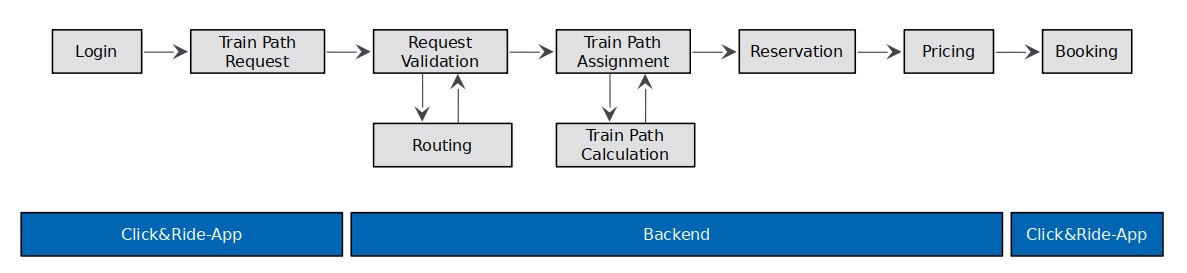
\includegraphics[width=\textwidth]{Bilder/process_sequence.jpg}
	% Else if you include an EPS file
	%    (it may need an interpreter for the PostScript language, e.g. Ghostscript),
	%\includegraphics[scale=0.30]{Fig1_Track.eps}
	\caption{Simplified process of Click\&Ride. The process is fully automated except for login and requesting a train path as well as booking.}
	\label{fig:process_sequence}
\end{figure}

Click\&Ride is a new B2B channel so only railway operators may use the functionalities. After logging in, the the train path request will be submitted to the back-end processes. Figure~\ref{fig:CnR_request} gives an impression of the user interface of Click\&Ride.
\begin{figure}[htb]
	\centering
	% If you include a JPG file,
	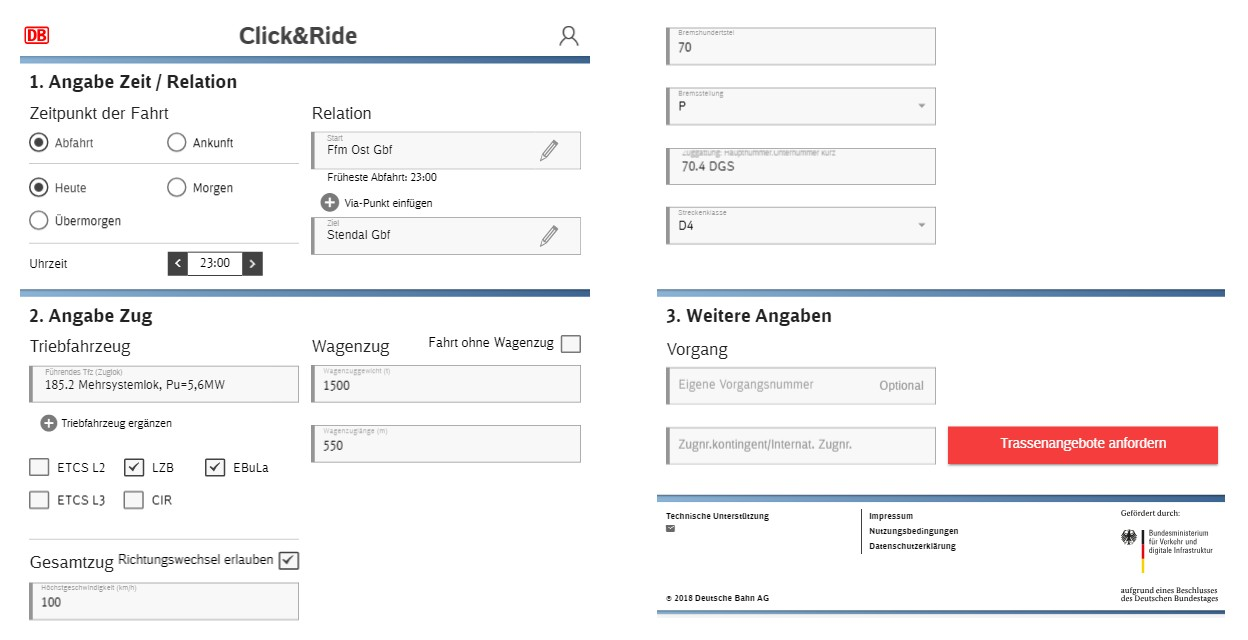
\includegraphics[width=\textwidth]{Bilder/request.jpg}
	% Else if you include an EPS file
	%    (it may need an interpreter for the PostScript language, e.g. Ghostscript),
	%\includegraphics[scale=0.30]{Fig1_Track.eps}
	\caption{GUI Click\&Ride to put a request. First the time requirements and waypoints need to be entered (upper left). Then the characteristics of the requested train need to be provided (lower left and upper right). Thirdly, in the lower right, there is space for additional information.}
	\label{fig:CnR_request}
\end{figure}

At first there is a validation service that ensures formal and technical fit to the tracks that will be used. For example an electric vehicle cannot use a track with no overhead line. If there are any problems with the train path request the railway operator gets instant feedback on the app's screen and can fix the problem. When there are no problems left the train path request is handled by the optimization in train path assignment (see Section~\ref{chap:Belegung}). If the technical properties of the requested train do not match the existing slots on the lines, a train path is generated automatically by train path calculation as described in Section~\ref{chap:Konstruktion}. Railway operators have a limited time to check the offered train path before booking. To make sure the capacity on the track cannot be given to other railway operators in the meanwhile, the train path is reserved for a maximum of ten minutes. To complete the response the total price for the train path is calculated and displayed in the Click\&Ride-App. An example response is shown in Figure~\ref{fig:CnR_response}.
\begin{figure}[htb]
	\centering
	% If you include a JPG file,
	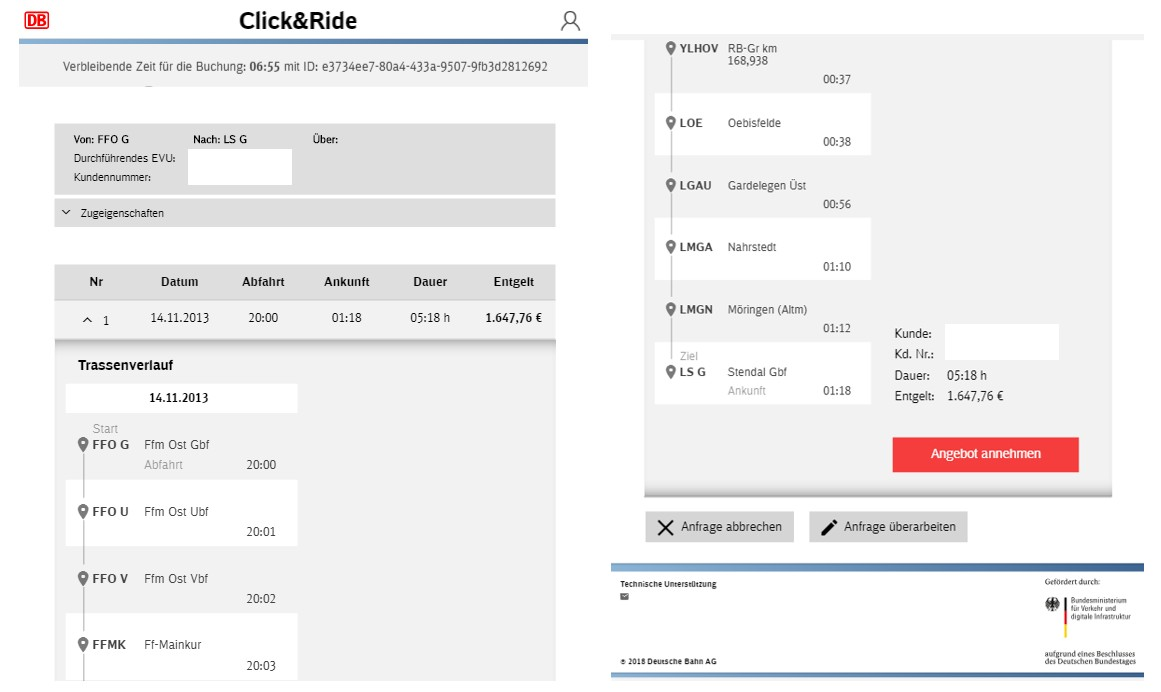
\includegraphics[width=\textwidth]{Bilder/response.jpg}
	% Else if you include an EPS file
	%    (it may need an interpreter for the PostScript language, e.g. Ghostscript),
	%\includegraphics[scale=0.30]{Fig1_Track.eps}
	\caption{Part of the response, i.e.\ a train path, to the request shown in Figure~\ref{fig:CnR_request}.}
	\label{fig:CnR_response}
\end{figure}

\subsubsection{Numerical Experiments}
For our experiments we use $1301$ real customer requests from November, 14th, 2013 in Germany. A customer request consists of the waypoints, time requirements and the characteristics of the train. The waypoints are at least the start of the request and its goal, but may also include some stops which should be served in between. The time requirements for our data consists only of an interval at the start of the request. But it is also possible to provide further time restrictions on the other waypoints. The characteristics of the request include all data necessary to calculate its dynamic properties such as acceleration and its static parameters like length, width and mass of the requested train. We consider the actual German infrastructure available in 2013. Furthermore, we also regard the blockages of passenger trains, which were scheduled on November, 14th, 2013 in order to have a realistic setup. We measure the quality of a train path in a metric called BFQ (\textit{Beförderungszeitquotient}) which is the travel time actually required by the train divided by the travel time that would have been necessary without additional stops. Note that for the Click \& Ride BFQ we use the shortest travel time on the shortest route in the denominator while the BFQ for the manual planners was calculated using the shortest travel time on the route chosen by the planner. This slight discrepancy in the numbers is to the advantage of the manual planners, as the route in the denominator could be longer.
%
\begin{table}[h]
	\centering
	\caption{Percentiles for response times, automatic BFQ and manual BFQ for $1301$ customer requests.}
	\label{tab:result_CnR}
	\begin{tabular}{lcccccc} \hline
	 	\textbf{Metric}    & $\textbf{50\%}$ & $\textbf{90\%}$ & $\textbf{95\%}$ & $\textbf{99\%}$ & \textbf{Max}  \\ \hline
		C\&R response time & $3.68$ sec.     & $50.28$ sec.    & $82.98$ sec.    & $147.89$ sec.   & $222.34$ sec. \\
		C\&R BFQ           & $1.03$          & $1.46$          & $1.73$          & $2.53$          & $6.07$ \\
		Manual BFQ         & $1.22$          & $1.94$          & $2.52$          & $4.35$          & $10.54$ \\ \hline
	\end{tabular}
\end{table}
\par

The experimental results, as provided in Table~\ref{tab:result_CnR}, show that $95\%$ of the request are served within $82.98$ seconds. $95\%$ of requests have a BFQ of at most $1.73$ while the same percentile had a BFQ of $2.52$ when planned manually. The maximal response time is $222.34$ seconds. Our target of serving a response in less than three minutes can be fulfilled in all but a few edge cases ($4$ out of the $1301$). This is a vast improvement compared to the up to three days required in the current manual process. The BFQ shows that the automatic process on average leads to faster train paths compared to the manual process.

\subsection{Annual Timetable}
\label{chap:Netzfahrplan}

The introduced methods will allow us to change the process of the creation of an annual timetable. In this use case all customer requests, for passenger and freight trains, are put at the same time and have to be provided with a timetable fulfilling all requests within $50$ days. This currently means a huge effort to DB Netz and can be eased by planning the freigth trains automatically. In an iterative process we manually create timetables for the passenger trains first. In the second step, the freight trains are calculated automatically with the methods described in Sections~\ref{chap:Konstruktion} and~\ref{chap:Belegung}. Afterwards the timetables are adapted and improved iteratively (compare Figure~\ref{fig:annual_planning} for a sketch of the process).

\begin{figure}[htb]
	\centering
	% If you include a JPG file,
	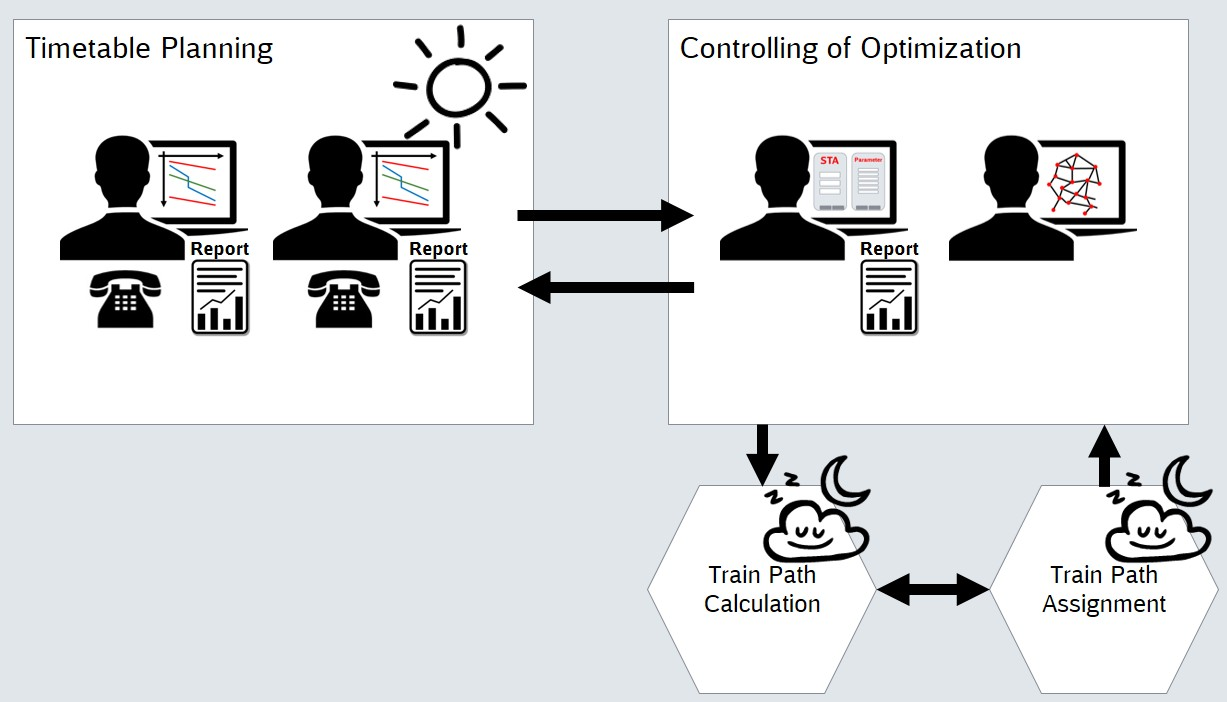
\includegraphics[width=\textwidth]{Bilder/annual_planning.jpg}
	% Else if you include an EPS file
	%    (it may need an interpreter for the PostScript language, e.g. Ghostscript),
	%\includegraphics[scale=0.30]{Fig1_Track.eps}
	\caption{Iterative Process for Annual Timetable: Planning by hand during the day and automated optimization during the night}
	\label{fig:annual_planning}
\end{figure}

\subsubsection{Numerical Experiments}
For this experiment we again consider the data from November, 14th, 2013 regarding infrastructure, blockages and customer requests. For clarity of presentation we restrict the shown results to the German part of Corridor One (\cite{Kor1}) rather than the entire German network. Corridor One stretches from sea ports of Rotterdam, Zeebrugge, Antwerp, Amsterdam and Vlissingen to the port of Genoa covering Netherlands, Belgium, Germany, Switzerland and Italy. Here only the part in Germany from Emmerich and Aachen to Basel will be considered. We have a test set consisting of 210 requests and create slots on 38 sections (compare Figure~\ref{fig:STAKarte}, left).
%As before a customer request consists of the waypoints, time requirements and the characteristics of the train.
%
\begin{table}[h]
	\centering
	\caption{Key performance indicators (KPIs) for the creation of slots}
	\label{tab:result_Netzfpl}
	\begin{tabular}{lcccc} \hline
		\textbf{KPIs}   					& \textbf{Result}  \\ \hline
		Number of slots             		& $935,814$                      \\
		computing time       				& 02:25h                     \\
		percentage rise Langerwehe (KLAW)   & $-1.70\%$                       \\
		percentage rise Bensheim (FBH) 		& $2.83\%$                       \\
		percentage rise Oberwesel (FOBW) 	& $6.82\%$                     \\ \hline
	\end{tabular}
\end{table}
\par

Table~\ref{tab:result_Netzfpl} shows the efficiency of our approach compared to human planer in 2013. While in average we are able to create about $3\%$ more slots, the biggest loss is $1.70\%$ in KLAW; contrasting a biggest gain of $6.82\%$ more slots in FOBW. Furthermore the creation of slots only takes $2.5$ hours compared to several days back in 2013.
%
\begin{table}[h]
	\centering
	\caption{Key performance indicators (KPIs) for the train path assignment}
	\label{tab:result_Netzfpl_Bel}
	\begin{tabular}{lcccc} \hline
		\textbf{KPIs}   							& \textbf{Result}  \\ \hline
		Number of Customer Requests     			& $210$                      \\
		computing time       						& 02:57h                     \\
		percentage train path assignments on slots  & $80\%$                       \\
		average BFQ 								& $1.27$                             \\ \hline
	\end{tabular}
\end{table}
\par

From Table~\ref{tab:result_Netzfpl_Bel} we see that precalculation of slots is beneficial for our approach as $80\%$ of all assigned train paths use slots. $20\%$ of the requests are assigned to individually created train paths. The average BFQ is $1.27$ which is more than $5\%$ better compared to the results of the manual process in 2013. As the train path assignment takes about $3$ hours, a whole timetable for Corridor One is created in $5.5$ hours fulfilling $210$ customers' requests on 935.814 slots.